\begin{myConceptSteps}{To determine if a relation consisting of a set of points is a function\dots}
    \myStep{inputs}{%
        Write down all the inputs ($x$ values).
    }
    \myStep{outputs}{%
        For each of the input values, {\bfseries\itshape write down} all of its outputs ($y$ values).
        To do this, you will have to look through all the points in the relation that have 
        that particular input value.
    }
    \myStep{count outputs}{%
        Ask ``Are any inputs with more than one output?''
        If the answer to that question is yes, 
        then the relation {\bfseries\itshape is not a function}.
        Otherwise, the relation {\bfseries\itshape is a function}.
    }
\end{myConceptSteps}




\begin{myExample}{
    Determine if this relation is a function. Explain your answer.
    \(
        \{ (1,2), (5,6), (3,4), (3,2) \}
    \)
}
    \vspace{1in}
\end{myExample}

\begin{myExample}{
    Determine if this relation is a function. Explain your answer.
    \begin{center}
    \begin{tabular}{cc}
            \toprule
            \emph{inputs} & \emph{outputs} \\
            \midrule
            1 & 2\\
            -5 & 3\\
            5 & -2\\
            1 & -3\\
            \bottomrule
    \end{tabular}
    \end{center}
}
    \vspace{1in}
\end{myExample}

\begin{myExample}{
    Find the domain and range of this function, and determine if it is a function. 
    Explain your answer.
    \begin{center}
    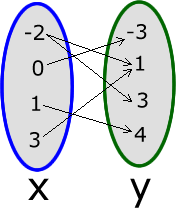
\includegraphics[width=2in]{../../common/images/domain-range-mapping.png}
    \end{center}
}
    \vspace{2.5in}
\end{myExample}
